% ch3.tex
% This work is licensed under the Creative Commons Attribution-Noncommercial-Share Alike 3.0 New Zealand License.
% To view a copy of this license, visit http://creativecommons.org/licenses/by-nc-sa/3.0/nz
% or send a letter to Creative Commons, 171 Second Street, Suite 300, San Francisco, California, 94105, USA.


\chapter{Turtles, and other slow moving creatures}\index{turtle}\label{ch:turtles}

There are certain similarities between turtles in the real world and a Python turtle.  In the real world, a turtle is a (sometimes) green reptile that moves around very slowly and carries its house on its back.  In the world of Python, a turtle is a small black arrow that moves very slowly around the screen. No mention of house-carrying though.

In fact, considering that a Python turtle leaves a trail as it moves around the screen, this makes it less like a real turtle, and more like a snail or a slug.  However, I suppose that a module called `slug' wouldn't be particularly attractive, so it makes sense to stick with turtles.  Just imagine the turtle is carrying a couple of marker pens with it, and drawing as it goes.

In the deep, dark, and distant past, there was a simple programming language called Logo.  Logo was used to control a robot turtle (called Irving).  Over time, the turtle evolved from a robot that could move around the floor, to a small arrow moving around a screen.

\emph{Which just goes to show, things don't always improve as technology advances---a little robot turtle would be a lot more fun.}

Python's turtle module (we'll come to modules a bit later, but for now just just think of a module as something we can use inside a program) is a little bit like the Logo programming language, but while Logo was (is) fairly limited, Python has many more capabilities.  The turtle module itself, is a useful way to learn how computers draw pictures on your computer screen.

Let's get started and see just how it works.  The first step is to tell Python we want to use turtle, by importing the module:

\begin{listing}
\begin{verbatim}
>>> import turtle
\end{verbatim}
\end{listing}

Then we need to display a canvas to draw on.  A canvas is just like the material an artist might use for painting; in this case it's a blank space for drawing on:

\begin{listing}
\begin{verbatim}
>>> t = turtle.Pen()
\end{verbatim}
\end{listing}

In this code, we call a special function (Pen\index{Pen}) on the module turtle, which automatically creates a canvas we can draw on.  A function is a re-useable piece of code (again we'll come to functions later) that does something useful---in this case, an object which represents the turtle is returned by the Pen function---we set that object to the variable `t' (in effect we're giving our turtle canvas the name `t'). When you type the code into the Python console, you'll see a blank box (the canvas) appear, looking something like figure~\ref{fig10}.

\begin{figure}
\begin{center}
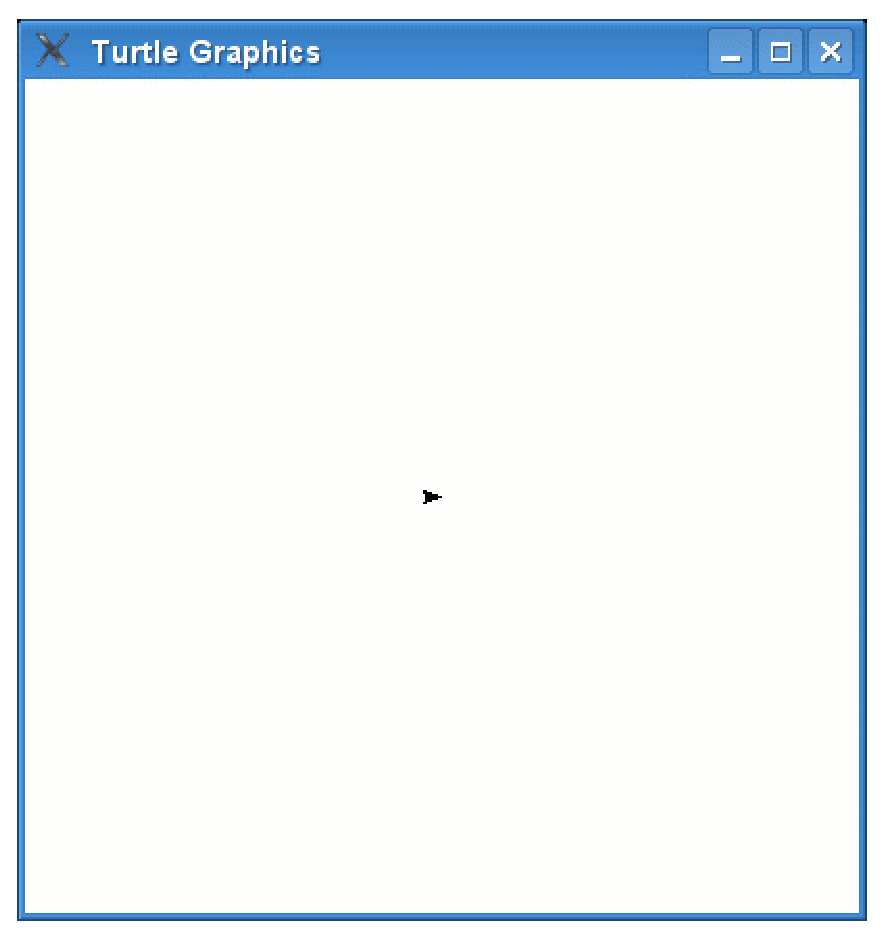
\includegraphics[width=72mm]{figure10.eps}
\end{center}
\caption{An arrow representing the turtle.}\label{fig10}
\end{figure}

\emph{Yes, that little arrow in the middle of the screen really is the turtle.  And, no, it's not very turtle-like.}

You can send instructions to the turtle, by using functions on the object that was created (by calling \code{turtle.Pen})---since we assigned that object to the variable \code{t}, we use \code{t} to send the instructions.
One turtle instruction is \code{forward}.  Forward\index{turtle!forward} tells the turtle to move forward in whatever direction she is facing (I have no idea whether it's a boy or a girl turtle, but let's just assume it's a girl-turtle for the moment). Let's tell the turtle to move forward 50 pixels (we'll talk about pixels in a minute):

\begin{listing}
\begin{verbatim}
>>> t.forward(50)
\end{verbatim}
\end{listing}

You should see something like figure~\ref{fig11}.

\begin{figure}
\begin{center}
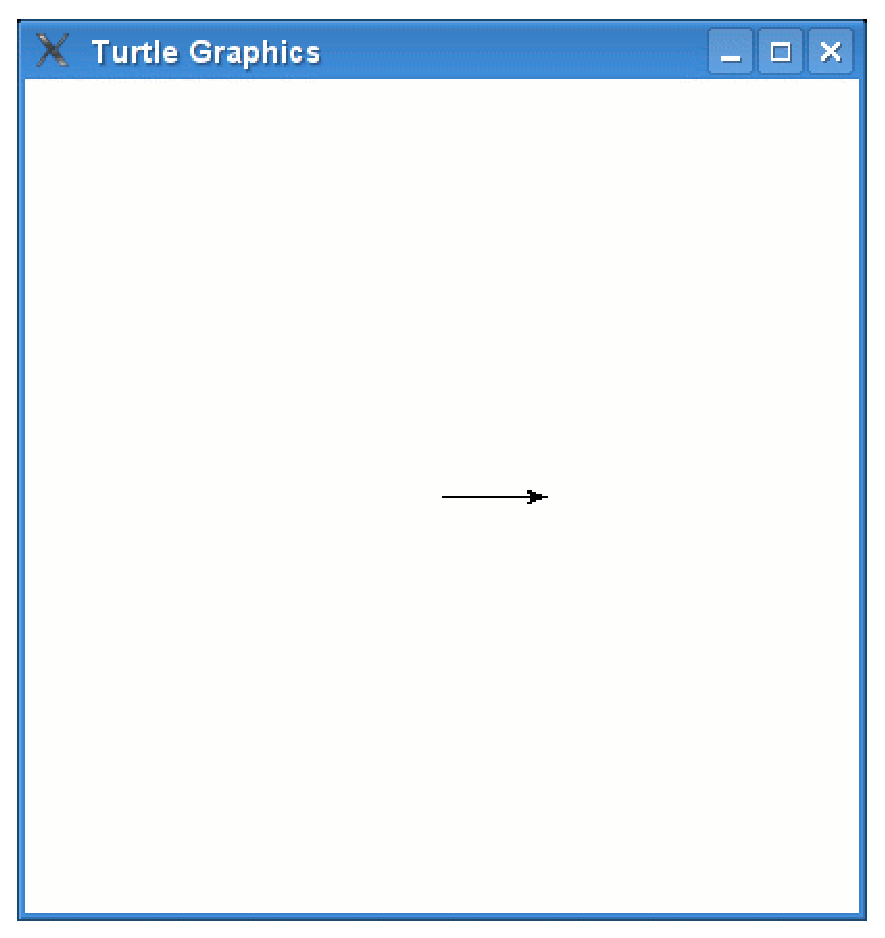
\includegraphics[width=72mm]{figure11.eps}
\end{center}
\caption{The turtle draws a line.}\label{fig11}
\end{figure}

From the turtle's point-of-view, she has moved forward 50 steps.  From our point-of-view, she has moved 50 pixels.

\noindent
\emph{So, what's a pixel?}

A pixel\index{pixels} is a dot on the screen.  When you look at your computer, everything is made up of tiny (square) dots.  The programs you use and the games you play on the computer, or with a Playstation, or an Xbox, or a Wii; are all made up of a whole bunch of different coloured dots, arranged on the screen.  In fact, if you look at your computer screen with a magnifying glass, you might just be able to make out some of those dots. So if we zoom in on the canvas and the line that was just drawn by the turtle, we can see the arrow representing the turtle, is also just a bunch of square dots, as you can see in figure~\ref{fig12}.

\begin{figure}
\begin{center}
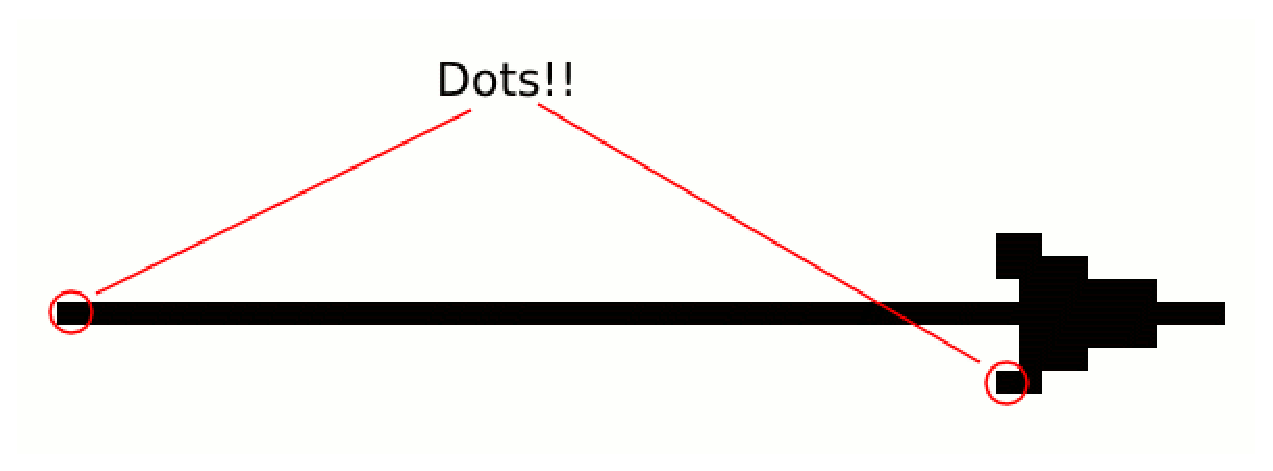
\includegraphics[width=72mm]{figure12.eps}
\end{center}
\caption{Zooming in on the line and the arrow.}\label{fig12}
\end{figure}

We'll talk more about these dots, or pixels, in a later chapter.

Next, we can tell the turtle to turn left\index{turtle!turning left} or right\index{turtle!turning right}:

\begin{listing}
\begin{verbatim}
>>> t.left(90)
\end{verbatim}
\end{listing}

This tells the turtle to turn left, 90 degrees.  You may not have learned about degrees\index{degrees} in school so far, but the easiest way to think about them, is that they are like the divisions on the face of a clock as seen in figure~\ref{fig13}.

\begin{figure}
\begin{center}
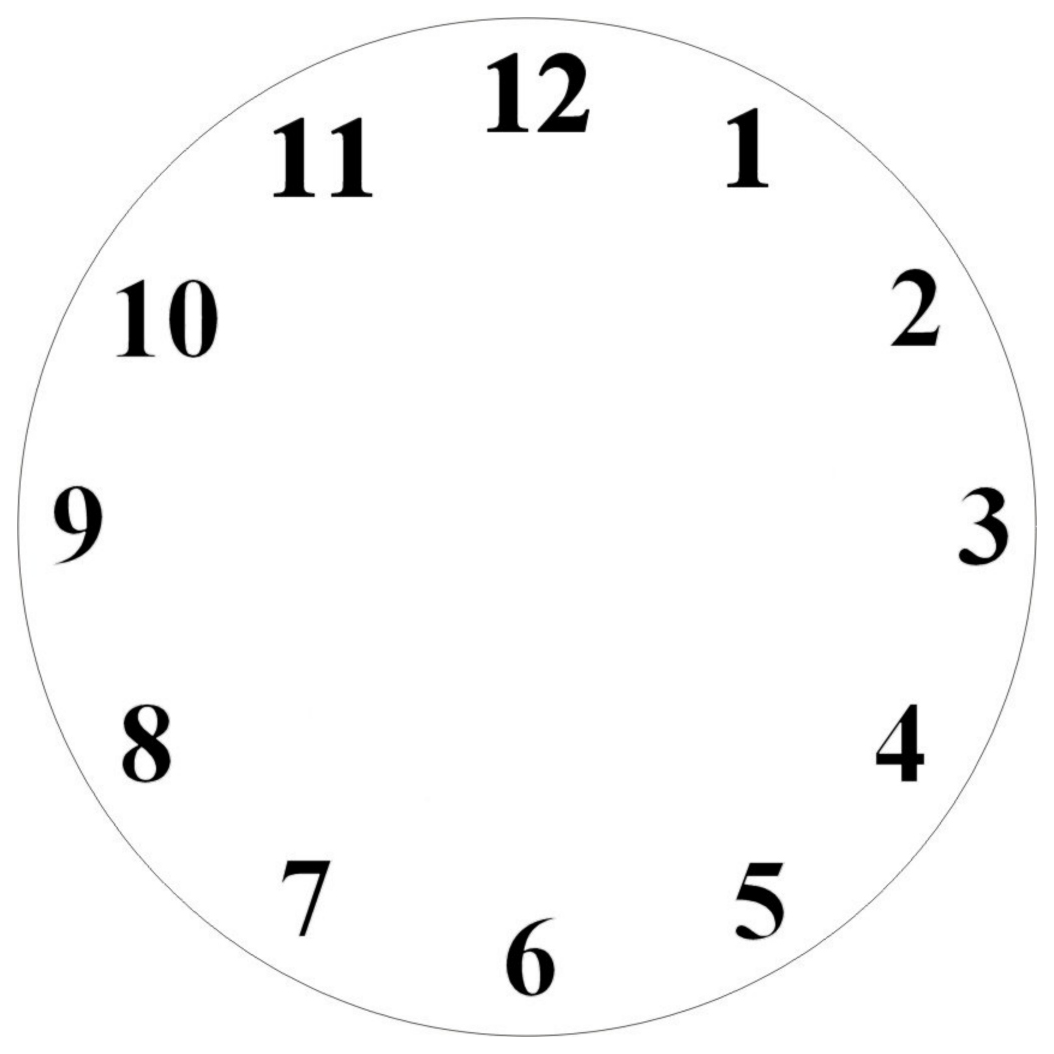
\includegraphics[width=52mm]{figure13.eps}
\end{center}
\caption{The `divisions' on a clock.}\label{fig13}
\end{figure}

The difference to a clock, is that rather than 12 divisions (or 60, if you're counting minutes rather than hours), there are 360 divisions.  So, if you count 360 divisions around the face of a clock, you get 90 where there's normally a 3, 180 where there's normally a 6, and 270 where there's normally a 9; and 0 would be at the top (at the start), where you normally see a 12.  Figure~\ref{fig14} shows you the degree divisions.

\begin{figure}
\begin{center}
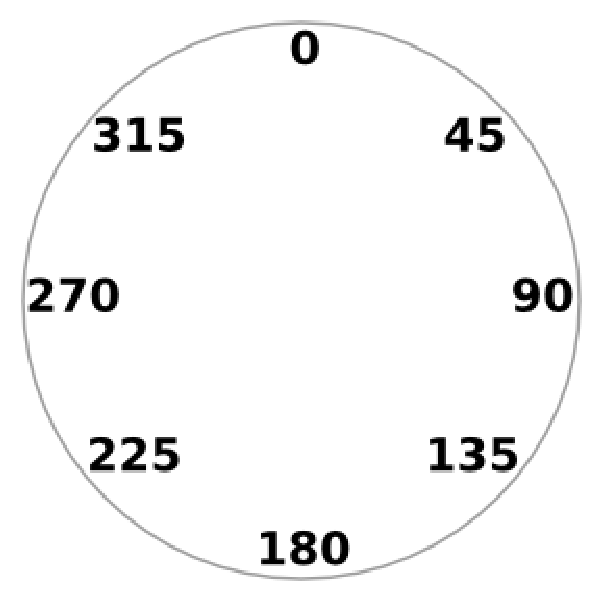
\includegraphics[width=52mm]{figure14.eps}
\end{center}
\caption{Degrees.}\label{fig14}
\end{figure}

So, what does it actually mean when you call \code{left(90)}?
\par
If you stand and face one direction, point your arm out directly away from your shoulder, THAT is 90 degrees.  If you point your left arm, that's 90 degrees left.  If you point your right arm, that's 90 degrees right.  When Python's turtle turns left, she plants her nose in one spot then swivels her body around the face the new direction (same as if you turned your body to face where your arm is pointing).  So, \code{t.left(90)} results in the arrow now pointing upwards, as shown in figure~\ref{fig15}.

\begin{figure}
\begin{center}
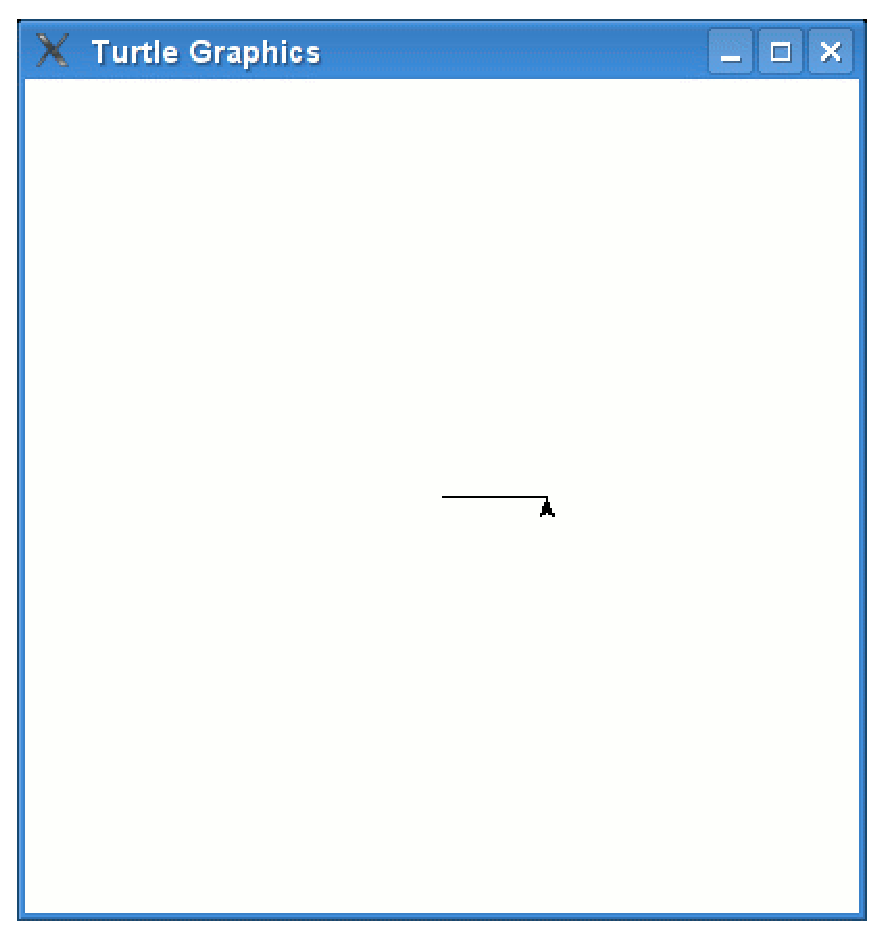
\includegraphics[width=72mm]{figure15.eps}
\end{center}
\caption{The turtle after turning left.}\label{fig15}
\end{figure}

Let's try the same commands again a few times:

\begin{listing}
\begin{verbatim}
>>> t.forward(50)
>>> t.left(90)
>>> t.forward(50)
>>> t.left(90)
>>> t.forward(50)
>>> t.left(90)
\end{verbatim}
\end{listing}

Our turtle has drawn a square and is left facing the same direction as she started (see figure~\ref{fig16}).

\begin{figure}
\begin{center}
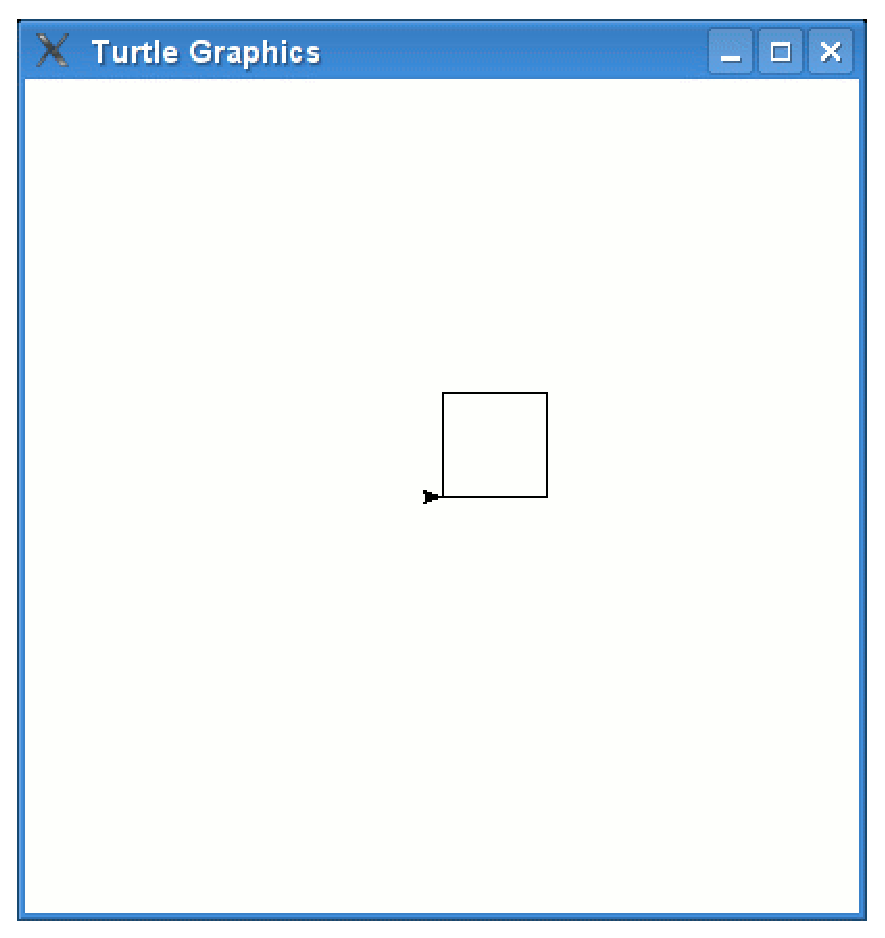
\includegraphics[width=72mm]{figure16.eps}
\end{center}
\caption{Drawing a square.}\label{fig16}
\end{figure}

We can erase what's on the canvas by using clear\index{turtle!clear}:

\begin{listing}
\begin{verbatim}
>>> t.clear()
\end{verbatim}
\end{listing}

Some of the other basic functions you can use with your turtle are: \code{reset}\index{turtle!reset}, which also clears the screen, but puts the turtle automatically back into her starting position; \code{backward}\index{turtle!backward}, which moves the turtle backwards; \code{right}, which turns the turtle to the right; \code{up}\index{turtle!up (stop drawing)} which tells the turtle to stop drawing as she moves (in other words pick her pen up off the canvas); and finally \code{down}\index{turtle!down (start drawing)} which tells the turtle to start drawing again. You call these functions in the same way we've used the others:

\begin{listing}
\begin{verbatim}
>>> t.reset()
>>> t.backward(100)
>>> t.right(90)
>>> t.up()
>>> t.down()
\end{verbatim}
\end{listing}

\noindent
We'll come back to the turtle module shortly.

\section{Things to try}

\emph{In this chapter we saw how to use turtle to draw simple lines, using left and right turns.  We saw that turtle uses degrees to turn, a bit like the minute divisions on a clock face.}

\subsection*{Exercise 1}
Create a canvas using turtle's \code{Pen} function, and draw a rectangle.

\subsection*{Exercise 2}
Create another canvas using turtles \code{Pen} function, and draw a triangle.

\newpage